\documentclass[11pt,a4paper]{article}
\usepackage[margin=24mm]{geometry}
\usepackage[T1]{fontenc}
\usepackage{lmodern,microtype,amsmath,amssymb,amsthm,graphicx,booktabs,array}
\usepackage[font=small,labelfont=bf]{caption}
\usepackage{xcolor}
\usepackage{xurl}
\usepackage[colorlinks=true,linkcolor=blue!45!black,citecolor=blue!45!black,urlcolor=blue!45!black]{hyperref}
\usepackage{enumitem,fancyhdr}
\setlist{nosep,leftmargin=*}
\setlength{\parskip}{1.5pt}
\linespread{0.97}
\setlength{\emergencystretch}{2em}
\newtheorem{theorem}{Theorem}
\newtheorem{lemma}{Lemma}
\newtheorem{corollary}{Corollary}
\newcommand{\D}{\mathcal{D}}
\newcommand{\C}{\mathcal{C}}
\newcommand{\U}{\mathcal{U}}
\newcommand{\mask}{\mathsf{MASK}}
\newcommand{\copyc}{\mathsf{COPY}}
\pagestyle{fancy}\fancyhf{}\fancyhead[L]{\small TraceMask}\fancyhead[R]{\small S. Gupta}\fancyfoot[C]{\thepage}
\setlength{\headheight}{14pt}
\title{\textbf{TraceMask: Earliest-Release Guarantees for Literal Redaction in Streaming AI Gateways}}
\author{Shivam Gupta\\Independent Researcher\\\small\href{mailto:shivam1720406@gmail.com}{shivam1720406@gmail.com}}
\hypersetup{pdftitle={TraceMask: Earliest-Release Guarantees for Literal Redaction in Streaming AI Gateways},pdfauthor={Shivam Gupta}}
\date{14 October 2026}
\begin{document}
\maketitle
\begin{abstract}
A streaming filter can recognize a secret correctly after part of it has already crossed the output boundary. Retaining a fixed suffix prevents this failure only under a suitable length bound, and can delay unrelated text. We study exact literal redaction: every source position covered by any occurrence of a registered string must be masked, and every other position must be preserved. For this policy, we characterize the longest irrevocably determined output prefix and derive an exact dictionary-specific bound on pending text. An Aho--Corasick implementation attains the release frontier using merged coverage intervals and linear amortized processing, without enumerating overlapping occurrences. In a controlled replay of 400 public instruction responses with inserted artificial secrets and five chunk schedules, TraceMask matches the offline policy in all 2,000 streams. Mean added delay falls from 83.31 to 15.68 input code points relative to a safe fixed buffer; the paired reduction is 67.64 [62.42, 72.76]. A simpler adaptive suffix buffer is nearly indistinguishable on this corpus, although a constructed overlap workload separates the methods. Exhaustive checks, saved decision traces, an independent verifier, and local HTTP/SSE tests support implementation correctness. A pinned third-party integration probe further separates buffering assumptions from UTF-8 decoding correctness. The contribution is a precise release contract and reproducible engineering study for known literal secrets, with no claim of general sensitive-entity detection or production prevalence.
\end{abstract}
\noindent\textbf{Keywords:} streaming inference; output redaction; online algorithms; finite-state matching; AI gateways; release latency

\section{Introduction}
A gateway forwards the first part of an answer containing a registered credential. The rest arrives in the next event. A detector subsequently finds the complete credential, but the gateway cannot retract the first part from the client, a log collector, or a text-to-speech service. Eventual detection and correct release are different properties.

This problem is established. Streaming redaction libraries retain tails, apply boundary guards, or buffer candidate runs; streaming moderation systems decide when to interrupt generated output \cite{sether,adr,frost,sentguard,streamguard}. The unresolved design question studied here is narrower: under a fully specified literal-masking policy, what text is still genuinely undecidable at a given prefix? A maximum-length buffer is safe when implemented with persistent coverage, but needlessly retains text that cannot belong to a future match. Even an adaptive buffer can retain positions already known to be masked.

Consider the dictionary $\D=\{\texttt{ab},\texttt{abcd}\}$. After observing \texttt{ab}, both positions must be masked whether the stream ends, continues with \texttt{cd}, or diverges. Retaining both characters merely because \texttt{ab} is a prefix of a longer secret delays decisions that are already final. After the next character \texttt{c}, however, its own decision remains unresolved: termination preserves it, while continuation with \texttt{d} masks it. This distinction depends on the union of completed match coverage and possible future coverage, rather than on suffix length alone.

We ask three questions. RQ1: Which source-coordinate decisions can be released without knowing the continuation? RQ2: What is the exact maximum pending text required by a given dictionary? RQ3: How much does this distinction matter in controlled instruction-response streams and at a real byte/event boundary?

Our contributions are (i) an explicit earliest-release characterization for union-of-occurrences masking; (ii) a finite, exact dictionary-specific pending bound; and (iii) a reference implementation and reproducible evaluation that distinguish correctness, delay, decoding, and termination. These are specialized results built on established automata and output-prefix ideas, not a claim to invent online matching or runtime enforcement. The empirical result is also qualified: most of the measured delay improvement comes from adaptive suffix recognition; exploiting known coverage adds little on the primary corpus.

\section{Related work and practical setting}
\paragraph{Matching and output transducers.}
Aho and Corasick provide persistent multi-pattern matching \cite{aho}. Sequential transducers and common-output-prefix constructions establish the general principle of moving determined output earlier \cite{mohri}. Rust's Aho--Corasick documentation explicitly distinguishes overlapping, standard, leftmost-first, and leftmost-longest semantics \cite{rustac}. Those semantics are consequential here: masking only a selected nonoverlapping match can leave part of an overlapping secret visible. We use the union of \emph{all} occurrence spans. The release theorem specializes common-output reasoning to this policy and gives a directly computable pending bound.

\paragraph{Runtime enforcement.}
Execution monitors and edit automata establish a formal basis for suppressing or transforming output \cite{schneider,ligatti}. Our transparency requirement is stronger than ``no literal appears in the final rendered string'': each covered source position is masked, while every uncovered position is copied. Otherwise, masking everything would solve the safety objective with no waiting, making any claimed latency optimum uninformative.

\paragraph{Streaming safeguards.}
Frost's release-boundary equivalence result concerns a deterministic stop policy for ordered conjunctive regular-language predicates \cite{frost}. It preserves the first withheld chunk. We instead transform the stream and determine when each source position can be copied or masked. SentGuard and StreamGuard address statistical semantic moderation at partial outputs \cite{sentguard,streamguard}; they do not supply the literal contract evaluated here. These approaches can be composed as separate controls, but their safety claims should not be substituted for one another.

\paragraph{Implementation evidence and commercial relevance.}
Sether offers streaming redaction, reversible placeholders, vaults, and application middleware \cite{sether}. Netresearch documents a fixed holdback approach in an LLM extension \cite{adr}. TinyVault documents literal output redaction and its limitations for transformed values \cite{tinyvault}. These public systems establish a practical integration need, not a market-size estimate or proof of unmet demand. A plausible application is a gateway that receives tenant-scoped literal credentials or protected phrases from a trusted registry, masks exact echoes before fan-out, and exposes release diagnostics. It complements entity detection and access controls. We do not claim customer validation, patentability, or that literal masking prevents semantic disclosure.

\begin{table}[t]
\centering\small
\caption{Positioning relative to the closest prior capabilities.}
\label{tab:related}
\begin{tabular}{>{\raggedright\arraybackslash}p{.23\linewidth}>{\raggedright\arraybackslash}p{.32\linewidth}>{\raggedright\arraybackslash}p{.35\linewidth}}
\toprule
Prior capability & Established functionality & Question addressed here\\\midrule
Aho--Corasick & Stateful recognition of literal occurrences & Which recognized or unresolved positions can be released?\\
Sequential transducers & Determined common output can be advanced & What is the closed-form frontier for union masking?\\
Streaming redaction & Tail buffering and practical boundary guards & What is the exact dictionary-specific pending requirement?\\
Release-time stop monitors & Withhold a policy-completing chunk & How can exact redaction continue streaming afterward?\\
Learned streaming guards & Statistical semantic risk assessment & How can a narrow literal contract be tested independently?\\\bottomrule
\end{tabular}
\end{table}

\section{Policy and observation model}
Let $\Sigma$ be a source alphabet and $\D\subset\Sigma^+$ a finite dictionary of nonempty strings. Positions are zero-based Unicode code-point indices in the implementation; no normalization or case folding is implicit. Empty dictionaries are allowed. Define the covered coordinates in a finite string $x$ by
\begin{equation}
\C_\D(x)=\bigcup_{p\in\D}\ \bigcup_{i:\ x[i:i+|p|]=p}[i,i+|p|),
\end{equation}
where intervals denote integer coordinate sets. The offline decision at coordinate $i$ is
\begin{equation}
R_\D(x)_i=\begin{cases}\mask,&i\in\C_\D(x),\\(\copyc,x_i),&\text{otherwise.}\end{cases}
\end{equation}
The output is a sequence of tagged decisions. A masked decision carries no source character. This avoids an ambiguity when the printable mask happens to equal a source character. Rendering one asterisk per masked code point is a separate presentation operation. The policy deliberately reveals length and location of redaction.

A streaming algorithm observes a growing prefix $x$ and can append decisions in source order. It cannot retract them. It is \emph{exact} if, on every successfully terminated finite input, its output equals $R_\D(x)$. Before successful termination, every emitted decision must agree with every finite continuation, including immediate termination. The generator and chunk partition may be adversarial. The dictionary, matcher, decoder, and release path are trusted and fixed for the logical stream.

Successful application termination is distinct from a broken connection. Our abort contract discards unresolved pending text. It guarantees that the already released prefix remains compatible with every continuation of the observed input. It does not reconstruct missing text, suppress all incomplete secret-like prefixes at a valid termination, or hide information conveyed by timing and output length.

\section{The earliest release frontier}
For a prefix $x$ of length $n$, let $d_\D(x)$ be the longest suffix of $x$ that is a \emph{proper} prefix of some dictionary member. Set $d_\D(x)=0$ if none exists. All possible future occurrences intersecting the observed prefix have starts represented by such suffixes. Their observed spans are nested, so their union is the single suffix interval
\begin{equation}
\U_\D(x)=[n-d_\D(x),n).
\end{equation}
Define
\begin{equation}\label{eq:frontier}
F_\D(x)=\min\bigl(\U_\D(x)\setminus\C_\D(x)\bigr),
\end{equation}
with the minimum of the empty set defined as $n$.

\begin{theorem}[Earliest exact release]\label{thm:frontier}
The longest prefix of source-coordinate decisions shared by $R_\D(xy)$ over all finite continuations $y\in\Sigma^*$ has length $F_\D(x)$. Therefore, an exact append-only algorithm can release all decisions before $F_\D(x)$, and no such algorithm can release coordinate $F_\D(x)$ when $F_\D(x)<n$.
\end{theorem}
\begin{proof}
A completed occurrence remains an occurrence after extension, so every coordinate in $\C_\D(x)$ is permanently masked. If a currently uncovered coordinate can become covered after extension, the covering occurrence must start before $n$ and end after $n$. Its observed portion is a suffix of $x$ that is a proper prefix of a dictionary member. Thus it lies within $\U_\D(x)$. Coordinates outside $\U_\D(x)$ that are currently uncovered remain copies under every extension.

Conversely, take an uncovered coordinate $i$ inside $\U_\D(x)$. The longest active suffix begins at $n-d_\D(x)$ and is a proper prefix of some $p\in\D$. Append the remaining part of $p$. The resulting occurrence covers every observed position in that suffix, including $i$. Immediate termination leaves $i$ uncovered. Hence its decision differs between two admissible completions. All coordinates before the first such $i$ are fixed; that coordinate is not. This is exactly Equation~\eqref{eq:frontier}.
\end{proof}

\paragraph{Why overlap matters.}
For $\D=\{\texttt{aba},\texttt{bab}\}$ and input \texttt{abab}, the occurrence spans cover all four coordinates. Selecting only the leftmost occurrence masks three. Our semantics avoids that leak by retaining coverage from all completed occurrences, even though the algorithm need only inspect the longest match ending at each position.

\subsection{An exact dictionary-specific pending bound}
Let $P(\D)$ be all proper prefixes of dictionary members, including the empty string. For $u\in P(\D)$, define $r_\D(u)$ as the first coordinate not in $\C_\D(u)$, or $|u|$ when every coordinate is covered.

\begin{theorem}[Exact pending bound]\label{thm:bound}
After processing any prefix and draining its earliest exact output, the maximum possible pending length is
\begin{equation}\label{eq:bound}
B(\D)=\max_{u\in P(\D)}\bigl(|u|-r_\D(u)\bigr).
\end{equation}
This maximum is attained by some proper dictionary prefix. If $L=\max_{p\in\D}|p|$, then $0\le B(\D)\le L-1$ for nonempty dictionaries; $B(\varnothing)=0$.
\end{theorem}
\begin{proof}
Given $x$, take its longest active suffix $u$, so $|u|=d_\D(x)$. Every occurrence contained entirely in $u$ also occurs in $x$ at its translated coordinates. Additional occurrences starting before $u$ may cover more of $u$, but cannot remove coverage. Therefore the first uncovered position in the active suffix is no earlier than $r_\D(u)$. By Theorem~\ref{thm:frontier}, the pending length is at most $|u|-r_\D(u)$; if no active suffix exists, it is zero.

For the reverse inequality, use input $x=u$ for a maximizing proper prefix. Its longest active suffix is the whole of $u$. Its first uncovered coordinate is exactly $r_\D(u)$, so its pending length equals the term in Equation~\eqref{eq:bound}. The bound by $L-1$ follows because a proper prefix has at most that length.
\end{proof}

The distinction can be large. With $\D=\{\texttt{a}^L\}$, $B=L-1$. With $\D=\{\texttt{a},\texttt{a}^{L-1}\texttt{b}\}$, every proper prefix of the long literal consists entirely of occurrences of \texttt{a}, and $B=0$. A longest-literal rule assigns the same buffer size to both dictionaries. The exact rule exposes why they need different pending state. This is a worst-case characterization for the declared coordinate policy, not a claim of zero processing or network latency.

\begin{figure}[t]
\centering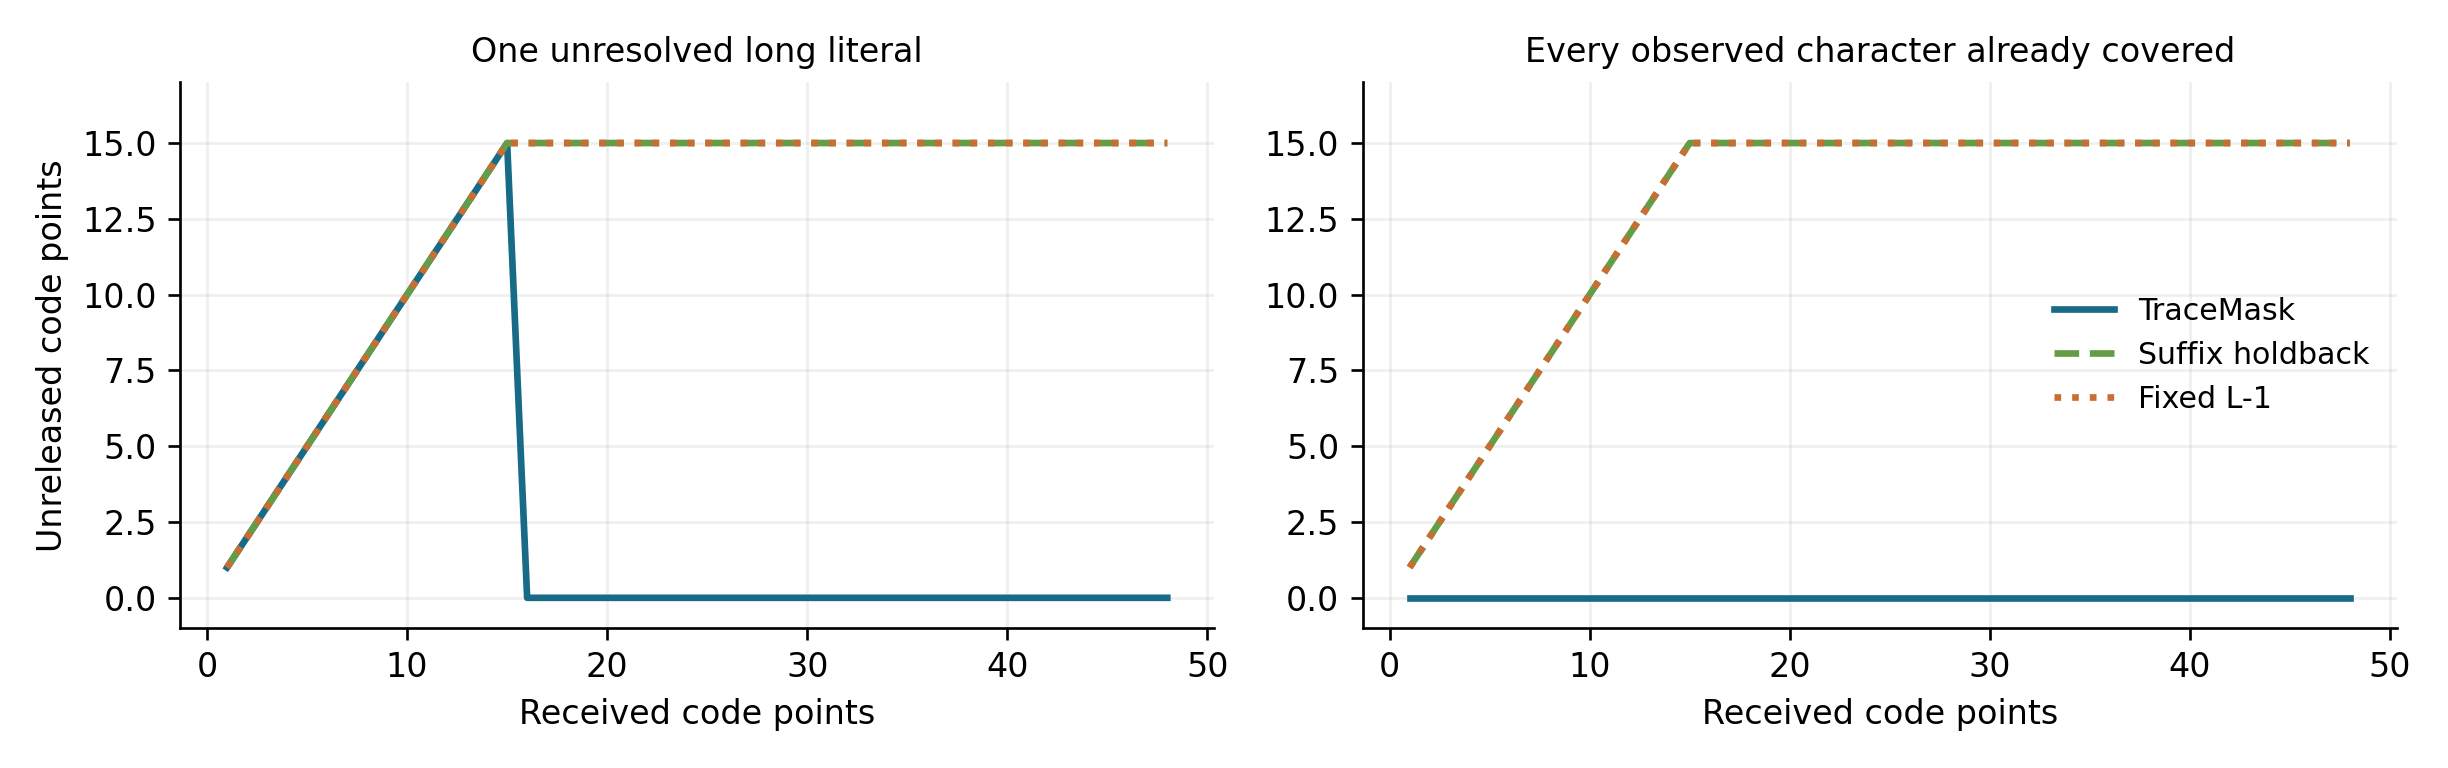
\includegraphics[width=\linewidth]{figures/pending_bounds.png}
\caption{Mechanism illustration with maximum literal length 16. Left: repeated \texttt{a} can become a single long secret, so decisions wait. Right: each \texttt{a} is already a complete registered secret, so TraceMask releases masks immediately. The suffix and fixed methods retain 15 code points. These are constructed examples.}
\label{fig:bounds}
\end{figure}

\section{Implementation}
\subsection{Matching without occurrence enumeration}
An Aho--Corasick trie stores a failure link, depth, longest terminal-match length reachable through failure links, and longest proper-prefix suffix length for each state. The latter is the current state's depth if it has a trie child; otherwise it inherits the value from its failure state. Terminal states with children can simultaneously represent a completed literal and a proper prefix of a longer one.

At each input code point, the longest completed match ending there contains every shorter match ending there. Marking just its interval therefore preserves the full union of coverage. Completed intervals arrive in increasing end-coordinate order. A deque merges overlapping intervals by removing overlapping intervals from its tail; obsolete intervals leave from its head. Each interval is inserted and removed at most once.

The pending source deque is drained in order. Its head is releasable when it is before the active-suffix interval, or when it is already covered. A covered head emits $\mask$ and discards the source character. A releasable uncovered head emits a copy. Repeating this operation stops exactly at Equation~\eqref{eq:frontier}. The algorithm preserves matching state across arbitrary input chunk boundaries.

\begin{figure}[t]
\centering\small
\begin{minipage}{.94\linewidth}
\hrule\vspace{5pt}
\textbf{Algorithm 1: process one code point $c$}\\
1. Append $c$ to pending; advance automaton; increment $n$.\\
2. Let $m$ be the longest completed match length in the current state.\\
3. If $m>0$, merge interval $[n-m,n)$ into pending match coverage.\\
4. Set $a=n-d$, where $d$ is the longest proper-prefix suffix length.\\
5. While the pending head is before $a$ or is covered:\\
\hspace*{12pt}emit its copy/mask decision and remove that source character.\\
6. Return decisions accumulated for the current caller's chunk.\vspace{5pt}\hrule
\end{minipage}
\caption{The release operation depends on both possible future matches and already completed coverage. Application success drains the remaining final decisions; abort discards them.}
\label{fig:algorithm}
\end{figure}

\paragraph{Complexity.}
Let $S$ be the number of trie states and $n$ the input length. With expected constant-time dictionary lookup, failure-link traversal is amortized linear in $n$. Longest-terminal metadata avoids a dependence on the number of overlapping matches. Interval merging and decision emission are also amortized $O(n)$. Shared automaton space is $O(S)$; retained source and coverage state are $O(B(\D)+1)$ per stream after draining, with a one-code-point transient. Returned output lists additionally require space proportional to the current emitted chunk. The optional exact-bound analyzer enumerates trie-prefix coverage in $O(SL)$ time. Its straightforward copied-array implementation may use $O(SL)$ auxiliary space; it is separate from the streaming path. The sparse failure-link construction used here also has a conservative $O(SL)$ preprocessing bound. These implementation bounds do not assert worst-case constant-time hash-table operations.

\subsection{The byte/event boundary and terminal contract}
The core accepts decoded strings, while a network supplies arbitrary bytes. Our JSON-over-SSE adapter performs strict incremental UTF-8 decoding, event framing, JSON decoding, schema validation, and only then literal masking. One adapter instance belongs to one logical stream. It recognizes \texttt{delta} events carrying exactly one string field and a \texttt{done} event carrying an empty object. It supports LF, CRLF, and CR line endings, comments, multiline data, and an initial UTF-8 byte-order mark. It is a constrained application adapter, not a complete provider SDK or reconnecting EventSource client. SSE's framing and UTF-8 requirements are specified independently by WHATWG \cite{sse}.

A successful \texttt{done} event permits final draining because immediate termination is now the declared continuation. A socket close without it causes an incomplete-stream error and discards pending text. Malformed UTF-8, invalid JSON, invalid event schemas, and event-size overflow also abort. Trailing line delimiters after \texttt{done} are accepted; subsequent data is rejected. A failed stream is never silently promoted to a successful completion. In particular, code that calls \texttt{finish()} from an unconditional cleanup block violates this adapter contract.

\begin{figure}[t]
\centering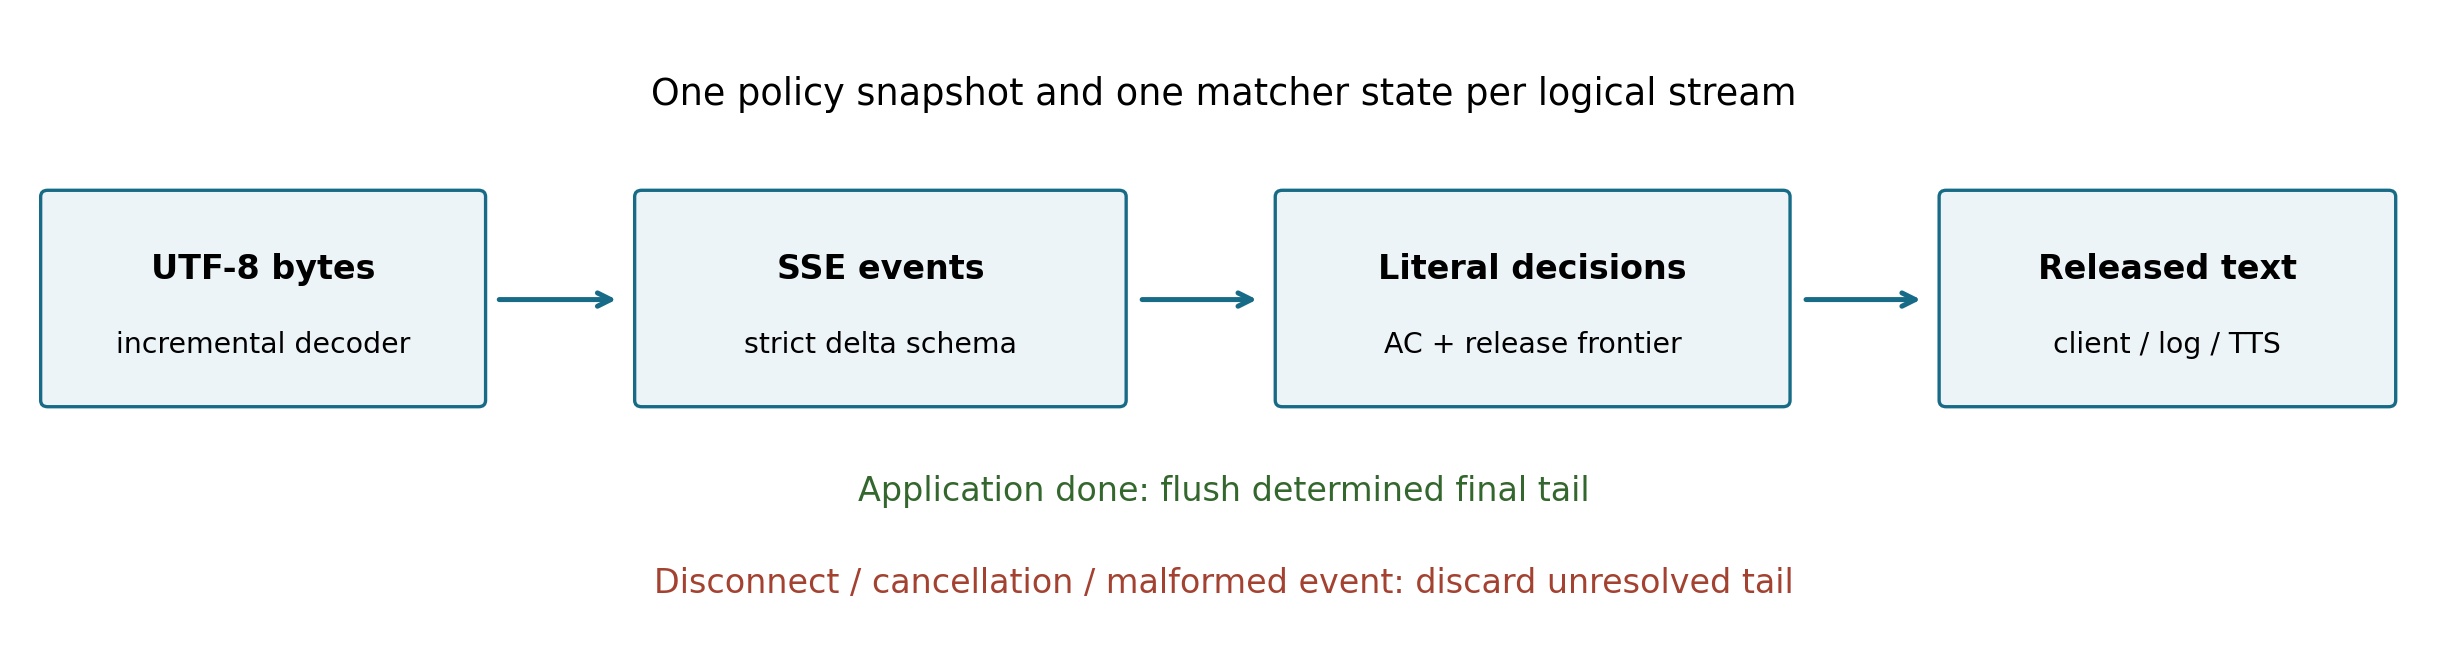
\includegraphics[width=\linewidth]{figures/gateway.png}
\caption{Reference integration boundary. Masking operates on logical decoded content, before any downstream fan-out. A transport EOF is not an application success signal. The event buffer is separately bounded and is not included in the literal core's pending bound.}
\label{fig:gateway}
\end{figure}

\section{Evaluation design}
\subsection{Frozen primary replay}
The protocol was written before the primary experiment; its hash and subsequent clarifications are included in the artifact. We sampled 400 responses with seed 1720406 from Databricks Dolly-15k \cite{dolly}. Of its 15,011 records, 7,119 have responses between 200 and 3,000 code points. Dolly responses supply public instruction-following text; they are not model generations in this experiment.

For each response we selected an artificial secret length from 16, 32, 64, 128, and 256 in a balanced cycle. Half are random ASCII identifiers and half are substrings sampled from the response. When a response is shorter than the chosen 256-character phrase length, its text is repeated before phrase selection. We insert the selected secret at the response midpoint with space delimiters and register three random same-length distractors. Natural phrase occurrences already present in the response also count under the oracle. This is a controlled echo workload, not an estimate of spontaneous secret leakage.

Each document is replayed with chunks of 1, 4, 16, and 64 code points and a seeded random schedule of 1--64 code points. The six methods yield 12,000 trials, including 2,000 per method. All trials are retained. Dictionaries, text, and chunk schedules are paired across methods.

\paragraph{Comparators.}
TraceMask uses the earliest frontier. \emph{Suffix holdback} uses the same matcher and coverage state but retains the entire longest active proper-prefix suffix, including positions already known to be masked. \emph{Fixed $L-1$} retains $L-1$ positions and persistent coverage. \emph{Fixed 32} uses the same mechanism with an insufficient lag for longer literals. \emph{Chunk-local} masks each chunk independently. \emph{Full response} delays all decisions until success. These are explicitly implemented baselines, not claims about commercial products. Persisting coverage is important: rescanning only the unmodified tail can lose the start of an already completed match after a partial release.

\paragraph{Metrics and uncertainty.}
For source position $i$, let $A_i$ be its arrival chunk's endpoint in input coordinates and $E_i$ the chunk endpoint at which its decision is returned. Added filter delay is $E_i-A_i$, in input code points. This excludes waiting caused purely by transport batching. It is neither milliseconds nor model tokens. We report document-macro mean delay, with chunk schedules averaged equally. A leaking coordinate is an oracle-covered position returned as a copy; overmasking is the reverse. Exact agreement requires both counts to be zero. Peak pending length is measured after each code point is processed and drained. Paired percentile intervals use 10,000 document bootstrap resamples, seed 2027. They quantify variation across sampled documents, not a probability of future failure.

\subsection{Mechanism and integration checks}
Exhaustive masking checks cover all nonempty subsets of binary patterns of length at most two and all binary texts of length at most eight: 32,193 dictionary/text cases. For 105 singleton or two-pattern dictionaries of maximum length three and binary prefixes through length six, an independent oracle enumerates continuations through length $L-1$, including immediate termination. The resulting 13,335 frontier cases test exact release length. Every future match intersecting a prefix can be completed within this continuation bound.

Additional checks include all 10,922 partitions of nonempty binary texts through length seven under a fixed overlapping dictionary, 2,000 seeded Unicode/random-dictionary cases, and 107 dictionary-bound cases including two long constructions. SSE tests examine 594 two-packet splits across all byte boundaries and three newline conventions, plus malformed inputs. A local HTTP server supplies 128 successful or interrupted streams over byte reads of sizes 1--64. These are fixture streams, not live model calls.

The supplemental local CPU profile uses Python 3.12.14 on an Apple M4 Pro with 24 GiB RAM, macOS 27.0.1. Each dictionary contains 4, 64, 512, or 4,096 random 24-character literals. We time construction and processing separately on the same 65,536-code-point nonmatching text with chunk size 16. One warm-up is excluded by design; all seven subsequent samples are retained. This is a single-process implementation profile, not a throughput or availability SLA.

\section{Results}
\subsection{Correctness and primary delay}
\begin{table}[t]
\centering\small
\caption{Primary replay: 2,000 streams per method. Delay is the document-macro mean added wait in input code points. Counts describe the constructed workload.}
\label{tab:primary}
\begin{tabular}{lrrrrr}\toprule
Method & Exact & Leaking & Leaked positions & Mean delay & Peak pending\\\midrule
TraceMask & 2,000 & 0 & 0 & 15.68 & 255\\
Suffix holdback & 2,000 & 0 & 0 & 15.68 & 255\\
Fixed $L-1$ & 2,000 & 0 & 0 & 83.31 & 255\\
Fixed 32 & 800 & 1,200 & 165,210 & 30.02 & 32\\
Chunk-local & 138 & 1,862 & 237,888 & 0.00 & 0\\
Full response & 2,000 & 0 & 0 & 336.48 & 3,117\\\bottomrule
\end{tabular}
\end{table}
All four safe methods match the offline policy in every primary trial (Table~\ref{tab:primary}). No method overmasks any source position in these trials. The short fixed buffer leaks in every tested stream whose registered literal length exceeds its useful lookahead; chunk-local processing fails whenever a protected occurrence spans an unfavorable chunk boundary. Their lower delays cannot be interpreted as safe performance improvements.

Relative to fixed $L-1$, TraceMask reduces macro mean added delay by 67.64 code points, with paired 95\% interval [62.42, 72.76], or 81.18\% of the comparator mean. Relative to full buffering, the reduction is 320.80 [299.12, 342.90]. Figure~\ref{fig:delay} shows dependence on literal length and type. Figure~\ref{fig:cdf} displays document-level heterogeneity. Full buffering additionally retains whole responses, while the longest literal is only 256 code points.

\begin{figure}[t]
\centering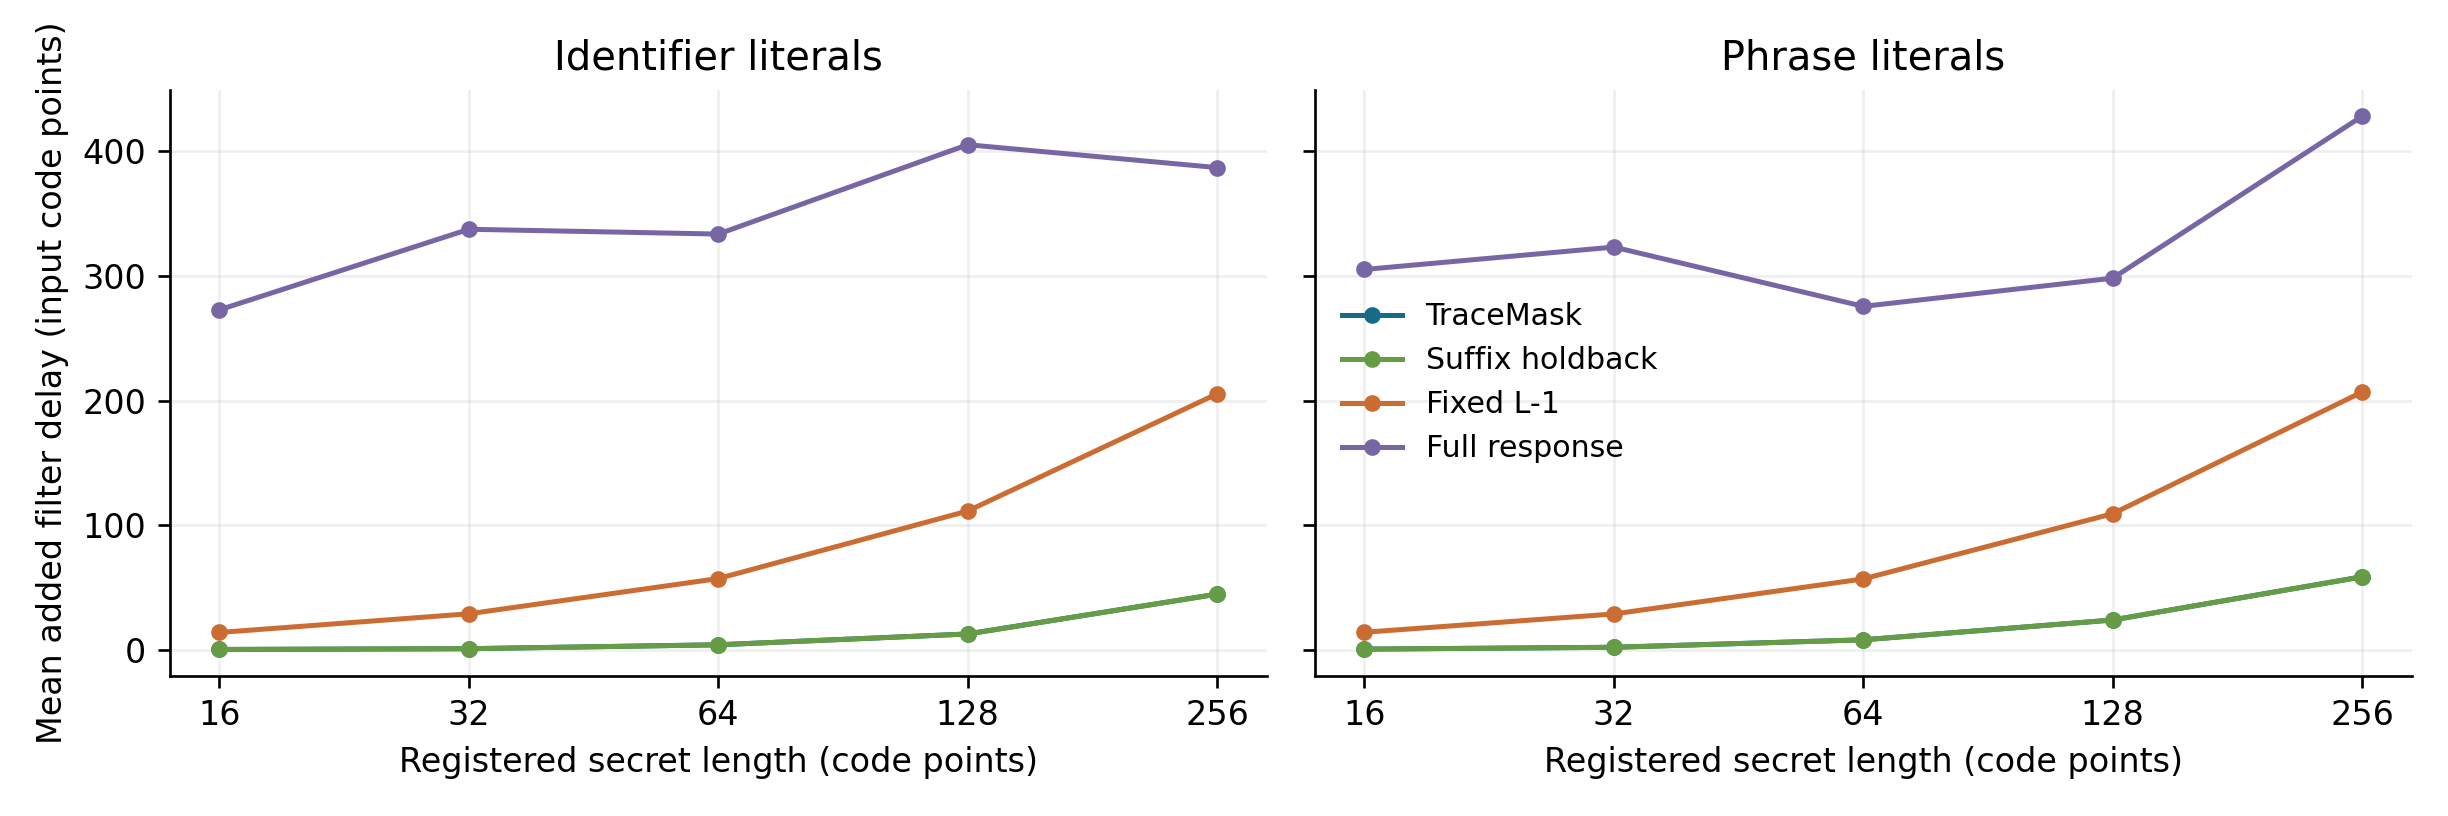
\includegraphics[width=\linewidth]{figures/delay_by_length.png}
\caption{Delay by secret type and registered length, averaged over all five chunk schedules. TraceMask and adaptive suffix holdback largely overlap. Random identifiers mainly create one long waiting interval; sampled phrases may also occur in the original answer.}
\label{fig:delay}
\end{figure}
\begin{figure}[t]
\centering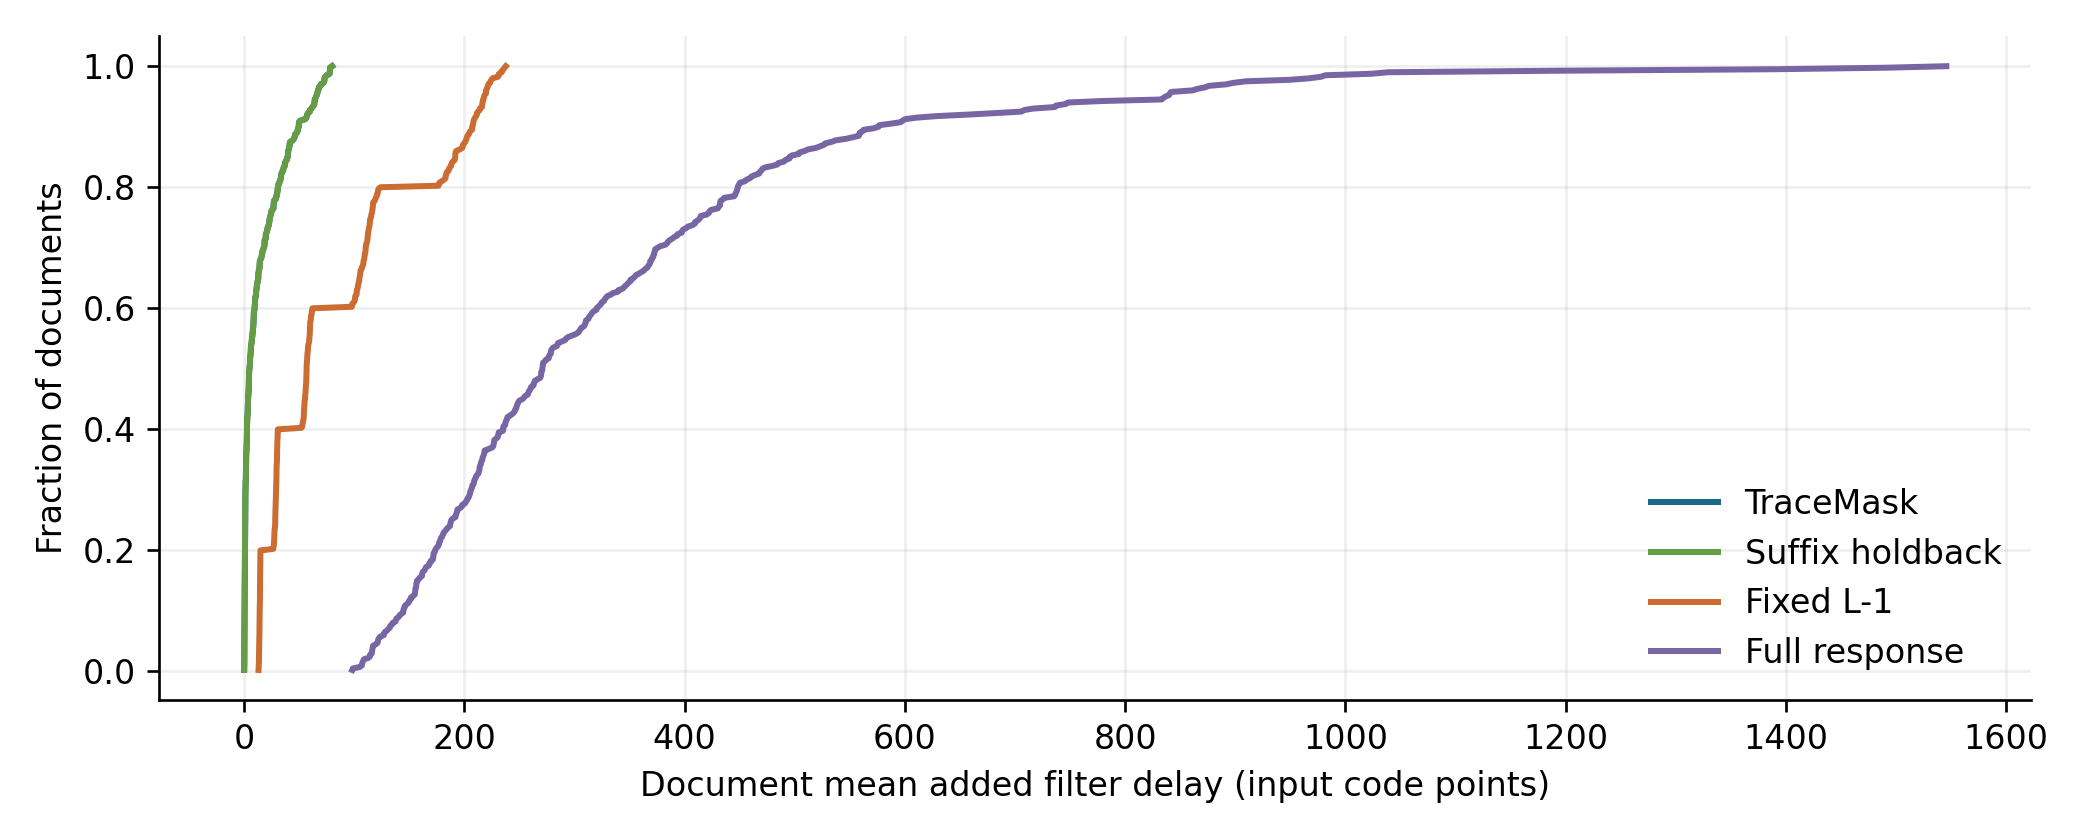
\includegraphics[width=.93\linewidth]{figures/delay_cdf.png}
\caption{Empirical cumulative distributions of document-macro added delay. The adaptive methods nearly coincide. The plot concerns artificial echo workloads, not observed production traffic.}
\label{fig:cdf}
\end{figure}

\paragraph{A small primary effect of coverage-aware release.}
Suffix holdback exceeds TraceMask by only 0.000751 code points on average, with paired interval [0.000313, 0.001382]. Although the interval excludes zero under this resampling procedure, the effect is operationally negligible on this corpus. Most of the gain over fixed buffering is therefore attributable to an established adaptive-prefix idea. The coverage-aware rule earns its role through its exact contract and dictionary-specific bound, rather than a large average empirical advantage here.

\subsection{Overlap construction and conformance}
For $\D=\{\texttt{a},\texttt{a}^{255}\texttt{b}\}$ and a stream of 65,536 \texttt{a} characters, TraceMask has zero added decision delay and zero post-drain pending characters. Suffix holdback and fixed 255 lag both retain up to 255 and have mean delay 254.50. Every output position is masked in all three methods. This construction verifies a large \emph{possible} separation, not its frequency in customer dictionaries.

All exhaustive output, enumerated-frontier, partition, random Unicode, and dictionary-bound checks pass. All 594 SSE byte-split cases and 128 local HTTP streams pass; interrupted fixtures emit only the safe public prefix and discard the unresolved secret prefix. An independently written verifier checks the saved masking coordinates and delay arithmetic for all 12,000 primary traces. These checks support the implementation; the proofs establish the universal statements within the mathematical model.

\subsection{Pinned third-party probe}
We also execute Sether 0.7.1 at commit \texttt{14ee74e2afca52c57f01ab43ee969db9d2429d0c}, using its public custom-detector interface \cite{sether}. The detector recognizes exactly one artificial literal; a deterministic placeholder is normalized to source-length masks for comparison. Four literals are tested at five UTF-8 byte chunk sizes, under the default 256 holdback and a length-based holdback: 40 cases in total. This tests buffering and decoding, not the accuracy of built-in detectors.

\begin{table}[t]
\centering\small
\caption{Supplemental Sether probe: exact agreement across five byte chunk sizes per setting. Inputs contain one controlled artificial literal.}
\label{tab:sether}
\begin{tabular}{>{\raggedright\arraybackslash}p{.30\linewidth}rr>{\raggedright\arraybackslash}p{.34\linewidth}}\toprule
Literal & Default 256 & Length bound & Interpretation\\\midrule
64-character identifier & 5/5 & 5/5 & Fits documented holdback assumptions.\\
1,024-character spaced phrase & 0/5 & 5/5 & A whitespace-run guard does not retain the whole phrase.\\
9,000-character identifier & 0/5 & 5/5 & Exceeds the default bounded candidate-run protection.\\
Unicode literal & 4/5 & 4/5 & One-byte buffers split UTF-8 before matching.\\\bottomrule
\end{tabular}
\end{table}
For the spaced phrase and long identifier, all 1,024 or 9,000 protected source positions are exposed under the default setting in each tested schedule. Increasing the holdback restores agreement for these ASCII cases. The package documents a bounded long-value protection rather than an unlimited guarantee; the 9,000-character case deliberately exercises the documented residual. In the Unicode case, one-byte buffer writes yield twelve replacement characters and defeat literal matching under either holdback. Other tested byte alignments happen to preserve the literal. Applying a correct incremental decoder before the string masker is therefore a separate obligation from choosing a sufficient buffer. These selected cases are not prevalence estimates, general comparisons of product quality, or evidence that built-in detectors promise arbitrary-length phrase protection.

\subsection{Local processing profile}
\begin{table}[t]
\centering\small
\caption{Supplemental reference implementation profile on one machine. Medians of seven recorded repetitions; 65,536 input code points, chunk size 16.}
\label{tab:timing}
\begin{tabular}{rrrrr}\toprule
Literals & Trie states & Build (ms) & Process (ms) & Peak pending\\\midrule
4 & 96 & 0.049 & 27.69 & 1\\
64 & 1,500 & 0.492 & 32.46 & 4\\
512 & 11,727 & 4.193 & 34.99 & 5\\
4,096 & 91,210 & 52.200 & 38.48 & 4\\\bottomrule
\end{tabular}
\end{table}
The local profile is consistent with processing that depends weakly on dictionary count once the matcher is built (Table~\ref{tab:timing}). Construction grows with trie size. These measurements do not establish superiority to a native matcher, GPU serving throughput, end-user latency, or multi-tenant capacity. Sharing an immutable automaton across streams avoids repeated compilation; policy changes require a new stream snapshot.

\section{Deployment implications and limitations}
\paragraph{Where the mechanism belongs.}
Masking must precede every untrusted sink that should receive redacted output. A guarded UI path does not protect a parallel raw log or speech path. Registry lookup, authorization, policy versioning, and stream ownership remain application responsibilities. The code masks exact decoded literals; escaped, normalized, case-altered, encoded, or paraphrased disclosures require explicit policy extensions or additional controls. A provider adapter must validate its own event schema and completion semantics; our fixture schema is intentionally small.

\paragraph{Choosing the simpler implementation.}
If a dictionary has few nested or overlapping literals, adaptive suffix holdback is an attractive default: it reproduces the exact final policy and nearly matches TraceMask's primary delay. Coverage-aware release is useful when minimizing the required pending text matters, when dictionaries contain substantial internal coverage, or when release-optimal behavior itself is the interface contract. The optional bound analyzer can identify the largest possible retention difference before deployment. A safe fixed buffer remains a reasonable implementation choice when its extra delay is acceptable and the maximum literal length is enforced.

\paragraph{Scope of evidence.}
The corpus contains deliberately inserted literal echoes, not unconstrained model outputs. Its identifier/phrase mixture, secret lengths, placement, and chunk schedules are experimental choices. They explain the observed delay distribution and cannot estimate customer leak rates. The bootstrap intervals do not quantify model uncertainty or security assurance. The overlap workload is chosen to expose the mechanism and is reported separately. The package probe uses one pinned library and custom literals. The timing profile excludes network, model generation, speech synthesis, allocation under high concurrency, and event parsing. We have not measured a commercial deployment or demonstrated a startup's demand.

\paragraph{Limits of the formal contract.}
Theorems assume a fixed finite dictionary, complete mediation, append-only ordered decisions, and exact code-point matching. They do not cover dynamic dictionary revocation, speculative downstream rendering, semantic entity recognition, or recovery of already released data. Successful termination intentionally preserves an incomplete unmatched prefix: it is not a complete registered occurrence. If a product requires hiding every sensitive prefix even at success, it needs a different offline policy and a new analysis. The visible mask preserves code-point count, not byte count, and reveals structural information. A time delay bound additionally requires assumptions on future input arrival; the pending-character bound alone provides no wall-clock guarantee during a stalled stream.

\section{Reproducibility and artifact}
The public artifact is available at \url{https://github.com/shi1720/tracemask}. It includes the core matcher, exact-bound analyzer, constrained SSE adapter, independent brute-force specifications, tests, frozen protocol, corpus generator, sampled corpus, all primary decision traces, local profile samples, third-party probe, figure scripts, and this manuscript's source. The derived corpus is attributed to Databricks and distributed under CC BY-SA 3.0; original code is MIT licensed. File hashes identify the input snapshot and result artifacts. No model API is needed to reproduce the reported experiments.

The primary evaluator and verifier are separate programs. The verifier does not import the production matcher. The raw trace records retain masked coordinates and per-position release delay, enabling independent recomputation of leakage, overmasking, and delay means. Tests of the exact frontier enumerate continuations rather than duplicating the streaming formula. Reproducibility instructions distinguish recorded-result verification from optional third-party reconstruction and from machine-dependent timing reruns.

\section{Conclusion}
Exact streaming redaction is a decision-release problem as well as a matching problem. For union-of-literal-occurrences masking, the first uncovered position in the longest active proper-prefix suffix is precisely where irrevocable output must stop. This yields both an earliest-release implementation and an exact dictionary-specific pending bound. Controlled replay shows a substantial advantage over safe fixed buffering, while also showing that a simpler adaptive baseline captures almost all of the average gain in this workload. The practical contribution is a testable contract connecting masking semantics, buffering, decoding, and application termination.

\begin{thebibliography}{99}\small
\bibitem{aho} A. V. Aho and M. J. Corasick. Efficient string matching: An aid to bibliographic search. \emph{Communications of the ACM}, 18(6):333--340, 1975. \url{https://doi.org/10.1145/360825.360855}.
\bibitem{mohri} M. Mohri. Finite-state transducers in language and speech processing. \emph{Computational Linguistics}, 23(2):269--311, 1997. \url{https://aclanthology.org/J97-2003/}.
\bibitem{schneider} F. B. Schneider. Enforceable security policies. \emph{ACM Transactions on Information and System Security}, 3(1):30--50, 2000. \url{https://doi.org/10.1145/353323.353382}.
\bibitem{ligatti} J. Ligatti, L. Bauer, and D. Walker. Edit automata: Enforcement mechanisms for run-time security policies. \emph{International Journal of Information Security}, 4:2--16, 2005. \url{https://users.ece.cmu.edu/~lbauer/papers/2005/ijis2005-editauto.pdf}.
\bibitem{rustac} A. Gallant and contributors. Aho--Corasick implementation design: Match semantics and streaming search. Software documentation. \url{https://github.com/BurntSushi/aho-corasick/blob/master/DESIGN.md}. Accessed 14 October 2026.
\bibitem{frost} C. M. Frost. Withholding the completing chunk: Exact release-boundary equivalence for production streaming guardrails. \emph{arXiv:2608.10279v2}, 2026. \url{https://arxiv.org/abs/2608.10279v2}.
\bibitem{sentguard} J. Yu, X. Wang, Y. Wang, J. Li, Y. Teng, X. Ma, and Y. Wang. SentGuard: Sentence-level streaming guardrails for large language models. \emph{arXiv:2606.02041}, 2026. \url{https://arxiv.org/abs/2606.02041}.
\bibitem{streamguard} P. Kavumba, K. Wataoka, H. H. Nguyen, J. Li, and M. Ohagi. Predict, don't react: Value-based safety forecasting for LLM streaming. \emph{arXiv:2604.03962}, 2026. \url{https://arxiv.org/abs/2604.03962}.
\bibitem{sether} G. Lebo and contributors. Sether 0.7.1: Streaming redaction implementation. Commit \texttt{14ee74e2afca52c57f01ab43ee969db9d2429d0c}. \url{https://github.com/raeven-co/sether}. Accessed 14 October 2026.
\bibitem{adr} Netresearch DTT GmbH. ADR-088: Live streaming redaction with a holdback buffer. 18 July 2026. \url{https://docs.typo3.org/p/netresearch/nr-llm/0.35/en-us/Adr/Adr088StreamingRedaction.html}.
\bibitem{tinyvault} TinyVault. Codemap integration: Literal-value output redaction. Product documentation. \url{https://www.tinyvault.dev/guide/codemap}. Accessed 14 October 2026.
\bibitem{dolly} Databricks. Databricks Dolly-15k. Dataset, 2023. CC BY-SA 3.0. \url{https://huggingface.co/datasets/databricks/databricks-dolly-15k}.
\bibitem{sse} WHATWG. HTML Living Standard, Section 9.2: Server-sent events. \url{https://html.spec.whatwg.org/multipage/server-sent-events.html}. Accessed 14 October 2026.
\end{thebibliography}

\appendix
\section{Artifact commands and verification targets}
Use Python 3.10 or newer for the core, and Python 3.11 or newer for the pinned analysis dependencies. The core requires only the standard library; analysis requires NumPy and Matplotlib. From the repository root:
\begin{quote}\small\ttfamily
python -m unittest discover -v\\
python experiments/verify.py\\
PYTHONPATH=. python experiments/run.py\\
PYTHONPATH=. python experiments/profile.py\\
PYTHONPATH=. python experiments/figures.py
\end{quote}
The evaluator can regenerate the frozen derived corpus from the original JSONL by passing its path. Input and protocol SHA-256 identifiers are listed below; line labels are not part of either hash.
\begin{quote}\footnotesize\ttfamily
Source JSONL:\\
2df9083338b4abd6bceb5635764dab5d833b393b55759dffb0959b6fcbf794ec\\
Frozen protocol:\\
2ec70a06cc1ac894152b8dcbb53663b73b62743fff7e31bbae4147a7db5c1789
\end{quote}
The artifact records subsequent supplemental diagnostics separately from the primary protocol.

The package probe requires checking out the pinned Sether revision, running its locked build, and passing the resulting \texttt{dist/index.js} path to \texttt{experiments/sether\_probe.mjs}. No third-party source is modified. Its output compares controlled ASCII leakage by aligned source positions; Unicode decoding failures are reported as exact-output mismatches and replacement-character counts, without pretending that changed-length output has an unambiguous source-coordinate leakage count.

\section{Why the dictionary-bound computation is finite}
For any observed prefix, possible future coverage of old coordinates is determined entirely by suffixes that are proper dictionary prefixes. These are trie nodes with children. To compute Equation~\eqref{eq:bound}, traverse the trie. Carry the matched-coverage vector for the root-to-node word, append an uncovered coordinate for each edge, and cover the final $m$ positions where $m$ is the longest terminal-match length at the resulting state. At every node with children, inspect the first uncovered coordinate. The maximum uncovered-tail length is $B(\D)$. Empty and fully covered words contribute zero.

This analyzer uses the same match metadata but is not itself the evidence for Theorem~\ref{thm:bound}. The test compares its result with maximum pending length over all binary texts through length seven for each of 105 dictionaries with literals of length at most three. Those texts include every proper-prefix witness and many contexts that could induce additional coverage. Separate long examples check $B=0$ and $B=L-1$. The proof explains why arbitrary longer contexts cannot exceed the computed value.
\end{document}
